%%%%%%%%%%%%%%%%%%%%%%%%%%%%%%%%%%%%%%%%%
% The Legrand Orange Book
% LaTeX Template
% Version 1.2 (19/5/13)
%
% This template has been downloaded from:
% http://www.LaTeXTemplates.com
%
% Original author:
% Mathias Legrand (legrand.mathias@gmail.com)
%
% License:
% CC BY-NC-SA 3.0 (http://creativecommons.org/licenses/by-nc-sa/3.0/)
%
% Compiling this template:
% This template uses biber for its bibliography and makeindex for its index.
% This means that to update the bibliography and index in this template you
% will need to run the following sequence of commands in the template
% directory:
%
% 1) pdflatex main
% 2) makeindex main.idx -s StyleInd.ist
% 3) biber main
% 4) pdflatex main
%
% This template also uses a number of packages which may need to be
% updated to the newest versions for the template to compile. It is strongly
% recommended you update your LaTeX distribution if you have any
% compilation errors.
%
% Important note:
% Chapter heading images should have a 2:1 width:height ratio,
% e.g. 920px width and 460px height.
%
%%%%%%%%%%%%%%%%%%%%%%%%%%%%%%%%%%%%%%%%%

%----------------------------------------------------------------------------------------
%	PACKAGES AND OTHER DOCUMENT CONFIGURATIONS
%----------------------------------------------------------------------------------------

\documentclass[11pt,fleqn]{book} % Default font size and left-justified equations

\usepackage[top=3cm,bottom=3cm,left=3.2cm,right=3.2cm,headsep=10pt,a4paper]{geometry} % Page margins
\usepackage{float}
\usepackage{xcolor} % Required for specifying colors by name
\definecolor{ocre}{RGB}{243,102,25} % Define the orange color used for highlighting throughout the book

% Font Settings
\usepackage{avant} % Use the Avantgarde font for headings
%\usepackage{times} % Use the Times font for headings
\usepackage{mathptmx} % Use the Adobe Times Roman as the default text font together with math symbols from the Sym­bol, Chancery and Com­puter Modern fonts

\usepackage{microtype} % Slightly tweak font spacing for aesthetics
\usepackage[utf8]{inputenc} % Required for including letters with accents
\usepackage[T1]{fontenc} % Use 8-bit encoding that has 256 glyphs

% Bibliography
\usepackage[style=alphabetic,sorting=nyt,sortcites=true,autopunct=true,babel=hyphen,hyperref=true,abbreviate=false,backref=true,backend=biber]{biblatex}
\addbibresource{bibliography.bib} % BibTeX bibliography file
\defbibheading{bibempty}{}

% Index
\usepackage{calc} % For simpler calculation - used for spacing the index letter headings correctly
\usepackage{makeidx} % Required to make an index
\makeindex % Tells LaTeX to create the files required for indexing

%----------------------------------------------------------------------------------------

%----------------------------------------------------------------------------------------
%	VARIOUS REQUIRED PACKAGES
%----------------------------------------------------------------------------------------

\usepackage{titlesec} % Allows customization of titles

\usepackage{graphicx} % Required for including pictures
\graphicspath{{./Pictures/}} % Specifies the directory where pictures are stored

\usepackage{lipsum} % Inserts dummy text

\usepackage{tikz} % Required for drawing custom shapes

\usepackage[english]{babel} % English language/hyphenation

\usepackage{enumitem} % Customize lists
\setlist{nolistsep} % Reduce spacing between bullet points and numbered lists

\usepackage{booktabs} % Required for nicer horizontal rules in tables

\usepackage{eso-pic} % Required for specifying an image background in the title page

%----------------------------------------------------------------------------------------
%	MAIN TABLE OF CONTENTS
%----------------------------------------------------------------------------------------

\usepackage{titletoc} % Required for manipulating the table of contents

\contentsmargin{0cm} % Removes the default margin
% Chapter text styling
\titlecontents{chapter}[1.25cm] % Indentation
{\addvspace{15pt}\large\sffamily\bfseries} % Spacing and font options for chapters
{\color{ocre!60}\contentslabel[\Large\thecontentslabel]{1.25cm}\color{ocre}} % Chapter number
{}  
{\color{ocre!60}\normalsize\sffamily\bfseries\;\titlerule*[.5pc]{.}\;\thecontentspage} % Page number
% Section text styling
\titlecontents{section}[1.25cm] % Indentation
{\addvspace{5pt}\sffamily\bfseries} % Spacing and font options for sections
{\contentslabel[\thecontentslabel]{1.25cm}} % Section number
{}
{\sffamily\hfill\color{black}\thecontentspage} % Page number
[]
% Subsection text styling
\titlecontents{subsection}[1.25cm] % Indentation
{\addvspace{1pt}\sffamily\small} % Spacing and font options for subsections
{\contentslabel[\thecontentslabel]{1.25cm}} % Subsection number
{}
{\sffamily\;\titlerule*[.5pc]{.}\;\thecontentspage} % Page number
[] 

%----------------------------------------------------------------------------------------
%	MINI TABLE OF CONTENTS IN CHAPTER HEADS
%----------------------------------------------------------------------------------------

% Section text styling
\titlecontents{lsection}[0em] % Indendating
{\footnotesize\sffamily} % Font settings
{}
{}
{}

% Subsection text styling
\titlecontents{lsubsection}[.5em] % Indentation
{\normalfont\footnotesize\sffamily} % Font settings
{}
{}
{}
 
%----------------------------------------------------------------------------------------
%	PAGE HEADERS
%----------------------------------------------------------------------------------------

\usepackage{fancyhdr} % Required for header and footer configuration

\pagestyle{fancy}
\renewcommand{\chaptermark}[1]{\markboth{\sffamily\normalsize\bfseries #1}{}} % Chapter text font settings
\renewcommand{\sectionmark}[1]{\markright{\sffamily\normalsize\thesection\hspace{5pt}#1}{}} % Section text font settings
\fancyhf{} \fancyhead[LE,RO]{\sffamily\normalsize\thepage} % Font setting for the page number in the header
\fancyhead[LO]{\rightmark} % Print the nearest section name on the left side of odd pages
\fancyhead[RE]{\leftmark} % Print the current chapter name on the right side of even pages
\renewcommand{\headrulewidth}{0.5pt} % Width of the rule under the header
\addtolength{\headheight}{2.5pt} % Increase the spacing around the header slightly
\renewcommand{\footrulewidth}{0pt} % Removes the rule in the footer
\fancypagestyle{plain}{\fancyhead{}\renewcommand{\headrulewidth}{0pt}} % Style for when a plain pagestyle is specified

% Removes the header from odd empty pages at the end of chapters
\makeatletter
\renewcommand{\cleardoublepage}{
\clearpage\ifodd\c@page\else
\hbox{}
\vspace*{\fill}
\thispagestyle{empty}
\newpage
\fi}

%----------------------------------------------------------------------------------------
%	THEOREM STYLES
%----------------------------------------------------------------------------------------

\usepackage{amsmath,amsfonts,amssymb,amsthm} % For including math equations, theorems, symbols, etc

\newcommand{\intoo}[2]{\mathopen{]}#1\,;#2\mathclose{[}}
\newcommand{\ud}{\mathop{\mathrm{{}d}}\mathopen{}}
\newcommand{\intff}[2]{\mathopen{[}#1\,;#2\mathclose{]}}
\newtheorem{notation}{Notation}[chapter]

\newtheoremstyle{ocrenum} % Theorem style name
{7pt} % Space above
{7pt} % Space below
{\normalfont} % Body font
{} % Indent amount
{\small\bf\sffamily\color{ocre}} % Theorem head font
{\;\;} % Punctuation after theorem head
{0.25em} % Space after theorem head
{\small\sffamily\color{ocre}\thmname{#1}\thmnumber{\@ifnotempty{#1}{ }\@upn{#2}} % Theorem text (e.g. Theorem 2.1)
\thmnote{\ {\the\thm@notefont\sffamily\bfseries\color{black}--- #3.}}} % Optional theorem note
\renewcommand{\qedsymbol}{$\blacksquare$} % Optional qed square

\newtheoremstyle{blacknumex} % Theorem style name
{7pt} % Space above
{7pt} % Space below
{\normalfont} % Body font
{} % Indent amount
{\small\bf\sffamily} % Theorem head font
{\;\;} % Punctuation after theorem head
{0.25em} % Space after theorem head
{\small\sffamily{\tiny\ensuremath{\blacksquare}}\ \thmname{#1}\thmnumber{\@ifnotempty{#1}{ }\@upn{#2}} % Theorem text (e.g. Theorem 2.1)
\thmnote{\ {\the\thm@notefont\sffamily\bfseries--- #3.}}} % Optional theorem note

\newtheoremstyle{blacknum} % Theorem style name
{7pt} % Space above
{7pt} % Space below
{\normalfont} % Body font
{} % Indent amount
{\small\bf\sffamily} % Theorem head font
{\;\;} % Punctuation after theorem head
{0.25em} % Space after theorem head
{\small\sffamily\thmname{#1}\thmnumber{\@ifnotempty{#1}{ }\@upn{#2}} % Theorem text (e.g. Theorem 2.1)
\thmnote{\ {\the\thm@notefont\sffamily\bfseries--- #3.}}} % Optional theorem note
\makeatother

% Defines the theorem text style for each type of theorem to one of the three styles above
\theoremstyle{ocrenum}
\newtheorem{theoremeT}{Theorem}[chapter]
\newtheorem{proposition}{Proposition}[chapter]
\newtheorem{problem}{Problem}[chapter]
\newtheorem{exerciseT}{Exercise}[chapter]
\theoremstyle{blacknumex}
\newtheorem{exampleT}{Example}[chapter]
\theoremstyle{blacknum}
\newtheorem{vocabulary}{Vocabulary}[chapter]
\newtheorem{definitionT}{Definition}[chapter]
\newtheorem{corollaryT}{Corollary}[chapter]

%----------------------------------------------------------------------------------------
%	DEFINITION OF COLORED BOXES
%----------------------------------------------------------------------------------------

\RequirePackage[framemethod=default]{mdframed} % Required for creating the theorem, definition, exercise and corollary boxes

% Theorem box
\newmdenv[skipabove=7pt,
skipbelow=7pt,
backgroundcolor=black!5,
linecolor=ocre,
innerleftmargin=5pt,
innerrightmargin=5pt,
innertopmargin=5pt,
leftmargin=0cm,
rightmargin=0cm,
innerbottommargin=5pt]{tBox}

% Exercise box	  
\newmdenv[skipabove=7pt,
skipbelow=7pt,
rightline=false,
leftline=true,
topline=false,
bottomline=false,
backgroundcolor=ocre!10,
linecolor=ocre,
innerleftmargin=5pt,
innerrightmargin=5pt,
innertopmargin=5pt,
innerbottommargin=5pt,
leftmargin=0cm,
rightmargin=0cm,
linewidth=4pt]{eBox}	

% Definition box
\newmdenv[skipabove=10pt,
skipbelow=10pt,
rightline=false,
leftline=true,
topline=false,
bottomline=false,
linecolor=ocre,
innerleftmargin=5pt,
innerrightmargin=5pt,
innertopmargin=0pt,
leftmargin=0cm,
rightmargin=0cm,
linewidth=4pt,
innerbottommargin=0pt]{dBox}	

% Corollary box
\newmdenv[skipabove=7pt,
skipbelow=7pt,
rightline=false,
leftline=true,
topline=false,
bottomline=false,
linecolor=gray,
backgroundcolor=black!5,
innerleftmargin=5pt,
innerrightmargin=5pt,
innertopmargin=5pt,
leftmargin=0cm,
rightmargin=0cm,
linewidth=4pt,
innerbottommargin=5pt]{cBox}				  
		  

% Creates an environment for each type of theorem and assigns it a theorem text style from the "Theorem Styles" section above and a colored box from above
\newenvironment{theorem}{\begin{tBox}\begin{theoremeT}}{\end{theoremeT}\end{tBox}}
\newenvironment{exercise}{\begin{eBox}\begin{exerciseT}}{\hfill{\color{ocre}\tiny\ensuremath{\blacksquare}}\end{exerciseT}\end{eBox}}				  
\newenvironment{definition}{\begin{dBox}\begin{definitionT}}{\end{definitionT}\end{dBox}}	
\newenvironment{example}{\begin{exampleT}}{\hfill{\tiny\ensuremath{\blacksquare}}\end{exampleT}}		
\newenvironment{corollary}{\begin{cBox}\begin{corollaryT}}{\end{corollaryT}\end{cBox}}	

%----------------------------------------------------------------------------------------
%	REMARK ENVIRONMENT
%----------------------------------------------------------------------------------------

\newenvironment{remark}{\par\vskip10pt\small % Vertical white space above the remark and smaller font size
\begin{list}{}{
\leftmargin=35pt % Indentation on the left
\rightmargin=25pt}\item\ignorespaces % Indentation on the right
\makebox[-2.5pt]{\begin{tikzpicture}[overlay]
\node[draw=ocre!60,line width=1pt,circle,fill=ocre!25,font=\sffamily\bfseries,inner sep=2pt,outer sep=0pt] at (-15pt,0pt){\textcolor{ocre}{R}};\end{tikzpicture}} % Orange R in a circle
\advance\baselineskip -1pt}{\end{list}\vskip5pt} % Tighter line spacing and white space after remark

%----------------------------------------------------------------------------------------
%	SECTION NUMBERING IN THE MARGIN
%----------------------------------------------------------------------------------------

\makeatletter
\renewcommand{\@seccntformat}[1]{\llap{\textcolor{ocre}{\csname the#1\endcsname}\hspace{1em}}}                    
\renewcommand{\section}{\@startsection{section}{1}{\z@}
{-4ex \@plus -1ex \@minus -.4ex}
{1ex \@plus.2ex }
{\normalfont\large\sffamily\bfseries}}
\renewcommand{\subsection}{\@startsection {subsection}{2}{\z@}
{-3ex \@plus -0.1ex \@minus -.4ex}
{0.5ex \@plus.2ex }
{\normalfont\sffamily\bfseries}}
\renewcommand{\subsubsection}{\@startsection {subsubsection}{3}{\z@}
{-2ex \@plus -0.1ex \@minus -.2ex}
{0.2ex \@plus.2ex }
{\normalfont\small\sffamily\bfseries}}                        
\renewcommand\paragraph{\@startsection{paragraph}{4}{\z@}
{-2ex \@plus-.2ex \@minus .2ex}
{0.1ex}
{\normalfont\small\sffamily\bfseries}}

%----------------------------------------------------------------------------------------
%	CHAPTER HEADINGS
%----------------------------------------------------------------------------------------

\newcommand{\thechapterimage}{}
\newcommand{\chapterimage}[1]{\renewcommand{\thechapterimage}{#1}}
\def\thechapter{\arabic{chapter}}
\def\@makechapterhead#1{
\thispagestyle{empty}
{\centering \normalfont\sffamily
\ifnum \c@secnumdepth >\m@ne
\if@mainmatter
\startcontents
\begin{tikzpicture}[remember picture,overlay]
\node at (current page.north west)
{\begin{tikzpicture}[remember picture,overlay]

\node[anchor=north west,inner sep=0pt] at (0,0) {\includegraphics[width=\paperwidth]{\thechapterimage}};

%Commenting the 3 lines below removes the small contents box in the chapter heading
\draw[fill=white,opacity=.6] (1cm,0) rectangle (8cm,-7cm);
\node[anchor=north west] at (1cm,.25cm) {\parbox[t][8cm][t]{6.5cm}{\huge\bfseries\flushleft \printcontents{l}{1}{\setcounter{tocdepth}{2}}}};

\draw[anchor=west] (5cm,-9cm) node [rounded corners=25pt,fill=white,fill opacity=.6,text opacity=1,draw=ocre,draw opacity=1,line width=2pt,inner sep=15pt]{\huge\sffamily\bfseries\textcolor{black}{\thechapter\ ---\ #1\vphantom{plPQq}\makebox[22cm]{}}};
\end{tikzpicture}};
\end{tikzpicture}}\par\vspace*{230\p@}
\fi
\fi
}
\def\@makeschapterhead#1{
\thispagestyle{empty}
{\centering \normalfont\sffamily
\ifnum \c@secnumdepth >\m@ne
\if@mainmatter
\startcontents
\begin{tikzpicture}[remember picture,overlay]
\node at (current page.north west)
{\begin{tikzpicture}[remember picture,overlay]
\node[anchor=north west] at (-4pt,4pt) {\includegraphics[width=\paperwidth]{\thechapterimage}};
\draw[anchor=west] (5cm,-9cm) node [rounded corners=25pt,fill=white,opacity=.7,inner sep=15.5pt]{\huge\sffamily\bfseries\textcolor{black}{\vphantom{plPQq}\makebox[22cm]{}}};
\draw[anchor=west] (5cm,-9cm) node [rounded corners=25pt,draw=ocre,line width=2pt,inner sep=15pt]{\huge\sffamily\bfseries\textcolor{black}{#1\vphantom{plPQq}\makebox[22cm]{}}};
\end{tikzpicture}};
\end{tikzpicture}}\par\vspace*{230\p@}
\fi
\fi
}
\makeatother % Insert the commands.tex file which contains the majority of the structure behind the template

\begin{document}

%----------------------------------------------------------------------------------------
%	Titulo
%----------------------------------------------------------------------------------------

\begingroup
\thispagestyle{empty}
\AddToShipoutPicture*{\put(6,5){
\includegraphics[scale=1]{background}}} % Image background
\centering
\vspace*{9cm}
\par\normalfont\fontsize{35}{35}\sffamily\selectfont
\centering
\includegraphics[scale=0.5]{icon640.png}

\centering
\includegraphics{i160x130.png}

Sudoku\par % Book title
\vspace*{1cm}
{\Huge Jefferson Rivera}\par % Author name
{\Huge Rubén Carvanal}\par % Author name
{\Huge César Madrid}\par % Author name
\endgroup

%----------------------------------------------------------------------------------------
%	COPYRIGHT PAGE
%----------------------------------------------------------------------------------------

\newpage
~\vfill
\thispagestyle{empty}

\noindent Copyright \copyright\ 2013 César Madrid\\ % Copyright notice

\noindent \textsc{Published by Publisher}\\ % Publisher

\noindent \textsc{book-website.com}\\ % URL

\noindent Licensed under the Creative Commons Attribution-NonCommercial 3.0 Unported License (the ``License''). You may not use this file except in compliance with the License. You may obtain a copy of the License at \url{http://creativecommons.org/licenses/by-nc/3.0}. Unless required by applicable law or agreed to in writing, software distributed under the License is distributed on an \textsc{``AS IS'' BASIS, WITHOUT WARRANTIES OR CONDITIONS OF ANY KIND}, either express or implied. See the License for the specific language governing permissions and limitations under the License.\\ % License information

\noindent \textit{Primera edicion, Julio 2013} % Printing/edition date

%----------------------------------------------------------------------------------------
%	TABLE OF CONTENTS
%----------------------------------------------------------------------------------------

\chapterimage{chapter_head_1.pdf} % Table of contents heading image

\pagestyle{empty} % No headers

\tableofcontents % Print the table of contents itself

\cleardoublepage % Forces the first chapter to start on an odd page so it's on the right

\pagestyle{fancy} % Print headers again

%----------------------------------------------------------------------------------------
%	Capitulo 1
%----------------------------------------------------------------------------------------

\chapterimage{chapter_head_2.pdf} % Chapter heading image

\chapter{Introduccion}

\section{Quienes somos?}\index{Paragraphs of Text}

Somos un grupo de tres estudiantes de Ingenieria en Ciencias Computacionales en la Escuela Superior Politecnica del Litoral, trabajamos en en proyecto para la materia Lenguajes de Programacion a cargo del profesor Javier Alejandro Tibau Benitez.


%------------------------------------------------

\section{Que es Sudoku?}\index{Paragraphs of Text}

"Sudoku es un pasatiempo que se publicó por primera vez a finales de la década de 1970 y se popularizó en Japón en 1986, dándose a conocer en el ámbito internacional en 2005 cuando numerosos periódicos empezaron a publicarlo en su sección de pasatiempos.El objetivo del sudoku es rellenar una cuadrícula de 9 x 9 celdas dividida en subcuadriculas de 3 x 3 (también llamadas "cajas" o "regiones") con las cifras del 1 al 9 partiendo de algunos números ya dispuestos en algunas de las celdas.  Aunque se podrían usar colores, letras, figuras, se conviene en usar números para mayor claridad, lo que importa, es que sean nueve elementos diferenciados, que no se deben repetir en una misma fila, columna o subcuadrícula. Un sudoku está bien planteado si la solución es única. La solución de un sudoku siempre es un cuadrado latino, aunque el recíproco en general no es cierto ya que el sudoku establece la restricción añadida de que no se puede repetir un mismo número en una región." \cite{http://es.wikipedia.org/wiki/Sudoku}


%------------------------------------------------

\section{Reglas de Juego}\index{Lists}

El sudoku se compone de 3 reglas basadas en el mismo punto, colocar numeros del 1 al 9 sin que se repitan en filas columnas y subcuadriculas.

Lists are useful to present information in a concise and/or ordered way\footnote{Footnote example...}.

\subsection{Filas}\index{Lists!Numbered List}

\begin{figure}[H]
\centering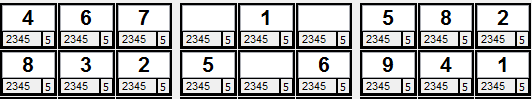
\includegraphics[scale=0.5]{ejfila1.png}
\caption{ejmeplo de sudoku}
\end{figure}

En la imagen se puede observar que en la primera fila pueden ir los numeros 9 y 3, mientras que en la segunda casilla solo encaja el 7 asi que es un número seguro a llenar

\begin{figure}[H]
\centering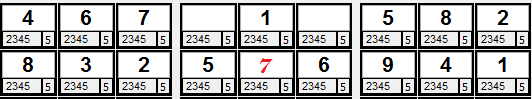
\includegraphics[scale=0.5]{ejfila.png}
\caption{ejmeplo de sudoku}
\end{figure}

\subsection{Columnas}\index{Lists!Numbered List}

\begin{figure}[H]
\centering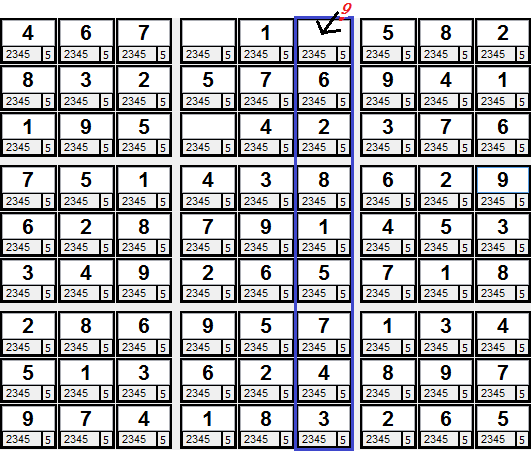
\includegraphics[scale=0.5]{ejcol.png}
\caption{ejmeplo de sudoku}
\end{figure}

En esta imagen se puede observar que en la columna indicada solo puede ir el número 9 asi que es un numero seguro a llenar.

\subsection{Subcuadriculas}\index{Lists!Numbered List}

\begin{figure}[H]
\centering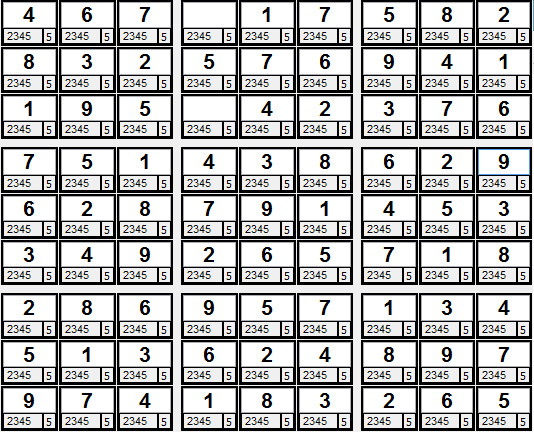
\includegraphics[scale=0.5]{ejsub.png}
\caption{ejmeplo de sudoku}
\end{figure}

En esta imagen observando la subcuadricula se nota que aun faltan 2 numeros por llenar, pero podemos observar que en la primera fila solo quedaun cuadro vacio con lo que aseguramos que ahi va un número 3, lo que nos deja la cuadricula con un espacio, donde cuadra el numero 8.

\begin{figure}[h]
\centering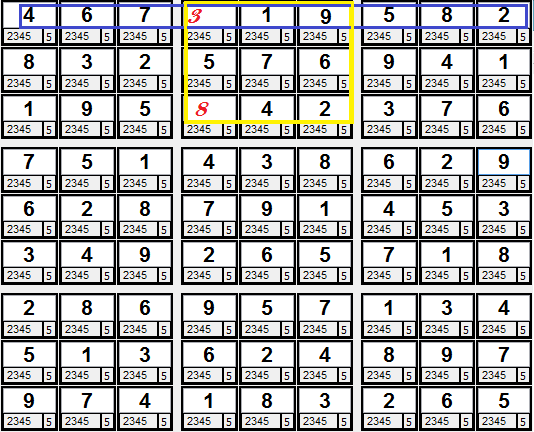
\includegraphics[scale=0.5]{ejsub1.png}
\caption{ejmeplo de sudoku}
\end{figure}


%----------------------------------------------------------------------------------------
%	Capitulo2
%----------------------------------------------------------------------------------------

\chapterimage{chapter_head_2.pdf} % Chapter heading image

\chapter{Arrancar la Aplicacion}

\section{Como abrir la aplicacion.}\index{Paragraphs of Text}

Para abrir nuestro juego debe ubircarse en la carpeta donde lo contiene y dependiendo de sus sistema operativo a abrira el programa indicado.



\subsection{Para windows.}\index{Lists!Numbered List}


En windows tienes que abrir el archivo llamado qsudoku.exe

\subsection{Para linux}\index{Lists!Numbered List}


En Linux arranca el archivo llamado qsudoku.gts




%----------------------------------------------------------------------------------------
%	Capitulo 3
%----------------------------------------------------------------------------------------

\chapterimage{chapter_head_2.pdf} % Chapter heading image

\chapter{Uso de la aplicacion}

\section{Seleccion de niveles}\index{Paragraphs of Text}

Una vez iniciada la aplicacion les va a mostrar las dificultades de juego, desde facil hasta modo leyenda, con las que podras ir demostrando tus habilidades de juego.

Selecciona una difiltudad segun su nivel de confianza en este juego .
\begin{enumerate}
\item Facil para principiantes y gente que nunca ha jugado antes.
\item Intermedio para gente que ya ha mejorado sus tecnicas y puede resolver los faciles mas rapido.
\item Profesional para gente ya con experiencia y ya tiene una habilidad para avanzar a este nivel.
\item Leyenda.- Se dice que hace mucho tiempo alguien logro terminar este sudoku (Juegalo bajo tu propio riesgo).
\end{enumerate}


%------------------------------------------------

\section{Inicio del juego y Nombre del Jugador}\index{Paragraphs of Text}

Una vez seleccionado el nivel de juego cargara una tabla de su sudoku y le pedira que ingrese su nombre. Una vez que lo ingrese arrancara el tiempo.
Para asignar valores a las casillas en blanco basta con dar click sobre la que desee editar y luego al lado izquiero cuenta con una botonera con los números del 1 al 9, el que seleccione se aplicara a su casilla.

\section{Jugando}\index{Lists!Numbered List}

Para asignar valores a las casillas en blanco basta con dar click sobre la que desee editar, esta casilla se pondra azul, y luego al lado derecho de la pantalla cuenta con una botonera con los números del 1 al 9, el que seleccione se aplicara a su casilla.

\section{Verificar Tablero}\index{Lists!Numbered List}

Cuando ud crea que ha armado un tablero correcto ud podra proceder a verificar que no tenga errores utilizando el boton "verificar" ubicado en el lado derecho sobre el cronometro.
En caso de que su sudoku tenga errores le saldra una advertencia y le marcara de rojo las casillas que no cumplan con las reglas, caso contrario le indicara que su sudoku esta correcto y terminara el juego.

\section{Guardar y Cargar partidas}\index{Lists!Numbered List}

\subsection{Guardar partidas}\index{Lists!Numbered List}

Si ud esta en media partida pero por alguna razon tiene que dejarla abandonada, ud puede utilizar la opcion de guardar partida, esta opcion se encuentra ubicada en el menu superior del juego -> Partida -> Guardar (o puede hacer uso del atajo rapido ctrl+g).

*imagen*

Estando ya en esa opcion le pedira que indique una ubicacion para guardar su partida, la selecciona y procede a guardar.

\subsection{Cargar partidas}\index{Lists!Numbered List}

Si ud desea continuar alguna partida que por alguna razon dejo abandonada pero la guardo, ud puede utilizar la opcion de cargar partida, esta opcion se encuentra ubicada en el menu superior del juego -> Partida -> Guardar (o puede hacer uso del atajo rapido ctrl+c).

*imagen*

Estando ya en esa opcion le pedira que indique la ubicacion donde guaro su partida, la selecciona y procede a abrirla.

\section{Salir del juego}\index{Lists!Numbered List}

En cualquier momento uds puede salir del juego ya sea usando la la X por defecto para cerrar programas en windows y linux o en el menu superior del juego -> Partida -> Salir.

Ud puede guardar su partida antes de cerrar el juego, si no lo hace esa partida quedara irrecuperable.





%----------------------------------------------------------------------------------------
%	Capitulo 4
%----------------------------------------------------------------------------------------

\chapterimage{chapter_head_2.pdf} % Chapter heading image

\chapter{Estructura de la pantalla de un juego}

\section{Partes de la pantallade juego}\index{Paragraphs of Text}

*imagen*


\begin{enumerate}
\item Tablero del sudoku(Filas, Columnas y subcuadriculas), donde se centra todo el juego.
\item Logo del de esta implementacion del juego.
\item Nombre del jugador.
\item Nivel del tablero.
\item Botoneras del 1 al 9 con las que se asigna el valor a las casillas.
\item Boton "verificar", para comprobar si tu sudoku esta correcto.
\item Cronometro(Tiempo que demora en resolver el sudoku).
\item Menu superior, donde puede Guardar/Cargar y encontrar informacion sobre el juego.

\end{enumerate}



%----------------------------------------------------------------------------------------
%	BIBLIOGRAPHY
%----------------------------------------------------------------------------------------

\chapter*{Bibliography}
\addcontentsline{toc}{chapter}{\textcolor{ocre}{Bibliography}}
\section*{Books}
\addcontentsline{toc}{section}{Books}
\printbibliography[heading=bibempty,type=book]
\section*{Articles}
\addcontentsline{toc}{section}{Articles}
\printbibliography[heading=bibempty,type=article]

%----------------------------------------------------------------------------------------
%	INDEX
%----------------------------------------------------------------------------------------

\cleardoublepage
\setlength{\columnsep}{0.75cm}
\addcontentsline{toc}{chapter}{\textcolor{ocre}{Index}}
\printindex

%----------------------------------------------------------------------------------------

\end{document}